\input{../../../.preambles/01-semester_work}
\input{../../../.preambles/10-russian}
\input{../../../.preambles/20-math}
\input{../../../.preambles/22-vectors}
\input{../../../.preambles/30-physics}
\usepackage{mathrsfs}

\newcommand{\ds}{\displaystyle}

\begin{document}
\maketitlepage{Факультет электроники и вычислительной техники}{физики}
{Электродинамика}{3}{}{студентка группы Ф-369\\Слоква~В.~И.}{f}
{доцент Грецов~М.~В.}{m}

\newpage
% ------------------------------------------------------------------------------
Задача 1.14: \emph{Определить поле плоского конденсатора, обкладки которого
равномерно заряжены с поверхностной плотностью зарядов \( +\sigma \) и
\( -\sigma \). Пространство между ними заполнено неоднородным диэлектриком,
проницаемость которого \( \eps = \eps(x) \). Краевым эффектом пренебречь. Ось
\( x \) направлена перпендикулярно к обкладкам от положительно заряженной
обкладки к отрицательной.}

\vspace*{2em}
\emph{Решение:}

\begin{minipage}{.4\textwidth}
    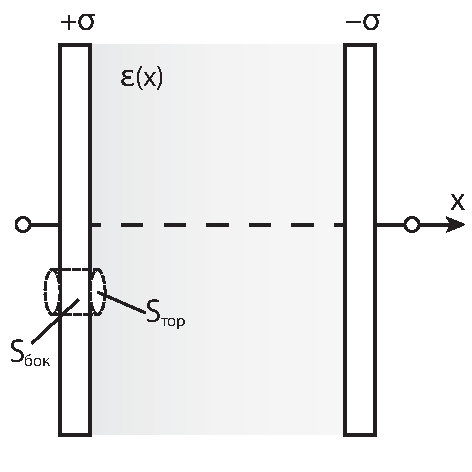
\includegraphics[width=\textwidth]{3-1}
\end{minipage}
\begin{minipage}{.55\textwidth}

Поля \( \vec{E} \) и \( \vec{D} \), в силу симметрии задачи, имеют только одну
компоненту и направлены вдоль оси \( x \).

Окружим малый участок пластины замкнутой цилиндрической поверхностью.
Запишем теорему Гаусса для \( \vec{D} \):
\[
    \oiint\limits_S \vec{D}\d\vec{S} = \sigma S_\emph{н.тор}
\]
\end{minipage}

Первый интеграл можно расписать следующим образом:
\[
    \oiint\limits_S \vec{D}\d\vec{S} = \iint\limits_{S_\emph{бок}} \vec{D}
    \d\vec{S} + \iint\limits_{S_\emph{н.тор}} \vec{D}\d\vec{S} +
    \iint\limits_{S_\emph{в.тор}} \vec{D}\d\vec{S}.
\]

Так как вне конденсатора поля нет, то \( \ds \iint\limits_{S_\emph{в.тор}}
\vec{D}\d\vec{S} = 0 \). Поле \( \vec{D} \) сонаправлено с осью \( x \),
следовательно, \( \ds \iint\limits_{S_\emph{бок}} \vec{D}\d\vec{S} = 0 \).

Тогда
\[
    \sigma S_\emph{н.тор} = \iint\limits_{S_\emph{н.тор}} \vec{D}\d\vec{S} =
    D\iint\limits_{S_\emph{н.тор}} dS = DS_\emph{н.тор},
\]
откуда \( D = \sigma \). С другой стороны \( D = \eps\Ezero E \), откуда
\( E = \cfrac{\sigma}{\eps\Ezero} \).

\vspace*{2em}
\emph{Ответ:} \( \vec{E} = \cfrac{\sigma}{\eps\Ezero}\,\vec{e}_x \).

\newpage
%-------------------------------------------------------------------------------
Задача 1.58: \emph{Вычислить емкость цилиндрического конденсатора. Длина его
\( l \), радиусы обкладок \( R_1 \) и \( R_2 \). Между обкладками два
коаксиальных слоя однородных диэлектриков с проницаемостью \( \eps_1 \) и
\( \eps_2 \), граница раздела между ними -- цилиндрическая поверхность радиуса
\( R_0 \). Краевым эффектом пренебречь.}

\vspace*{2em}
\emph{Решение:}

\begin{minipage}{.4\textwidth}
    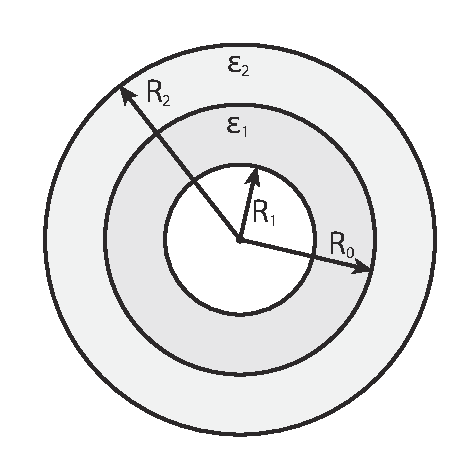
\includegraphics[width=\textwidth]{3-2}
\end{minipage}
\begin{minipage}{.55\textwidth}
    Пусть конденсатор заряжен с погонным зарядом \( \gamma = q/2\pi r \).
    
    Поле \( \vec{E} \) между обкладками создается только внутренним цилиндром
    \[
        E(r)\Bigr|_{R_1 < r < R_2} = \frac{\gamma}{2\pi\eps\Ezero r}\biggr|_{R_1 < r < R_2}.
    \]
    
    По теореме Гаусса:
    \[
        \oiint\limits_S \vec{E}\d\vec{S} = \frac{q}{\eps\Ezero}
    \]
\end{minipage}
    
Первый интеграл можно расписать следующим образом:
\[
    \oiint\limits_S \vec{E}\d\vec{S} = \iint\limits_{S_\emph{бок}} \vec{E}
    \d\vec{S} + 2\iint\limits_{S_\emph{тор}} \vec{E}\d\vec{S}.
\]
Так как поле \( \vec{E} \uparrow\uparrow \vec{n}_\emph{бок} \), то
\( \ds \iint\limits_{S_\emph{тор}} \vec{E}\d\vec{S} = 0 \) и
\( \ds \iint\limits_{S_\emph{бок}} \vec{E}\d\vec{S} =
E\iint\limits_{S_\emph{бок}} dS = 2\pi rlE \).

Тогда поле \( E = \cfrac{q}{2\pi rl \eps\Ezero} \), и разность потенциалов:
\begin{gather*}
    \Delta\phi = \int\limits_{R_1}^{R_2} E\,dr = \frac{q}{2\pi\Ezero l}\left(
    \int\limits_{R_1}^{R_0} \frac{dr}{\eps_1r} + \int\limits_{R_0}^{R_2} \frac{dr}
    {\eps_2r}\right) = \frac{q}{2\pi\Ezero l}\left(\frac{1}{\eps_1} \ln R
    \biggr|_{R_1}^{R_0} + \frac{1}{\eps_2}\ln R\biggr|_{R_0}^{R_2}\right) = \\
    = \frac{q}{2\pi\Ezero l}\left(\frac{1}{\eps_1}\ln\frac{R_0}{R_1} +
    \frac{1}{\eps_2}\ln\frac{R_2}{R_0}\right).
\end{gather*}

Тогда емкость цилиндрического конденсатора: \( \ds C = \frac{q}{\Delta\phi} =
\frac{2\pi\Ezero l}{\left(\frac{1}{\eps_1}\ln\frac{R_0}{R_1} + \frac{1}{\eps_2}
\ln\frac{R_2}{R_0}\right)} \).

\emph{Ответ:} \( \ds C =\frac{2\pi\Ezero l}{\left(\frac{1}{\eps_1}
\ln\frac{R_0}{R_1} + \frac{1}{\eps_2}\ln\frac{R_2}{R_0}\right)} \).

\newpage
%-------------------------------------------------------------------------------
Задача 1.115: \emph{В вакууме имеется бесконечно длинный заземленный проводящий
круглый цилиндр радиуса \( a \). Параллельно его оси протянута нить на
расстоянии \( l > a \) от нее. Нить равномерно заряжена с линейной плотностью
\( \chi \). Определить создаваемое ею поле и силу, действующую на единицу длины
нити.}

\vspace*{2em}
\emph{Решение:}

\begin{minipage}{.5\textwidth}
    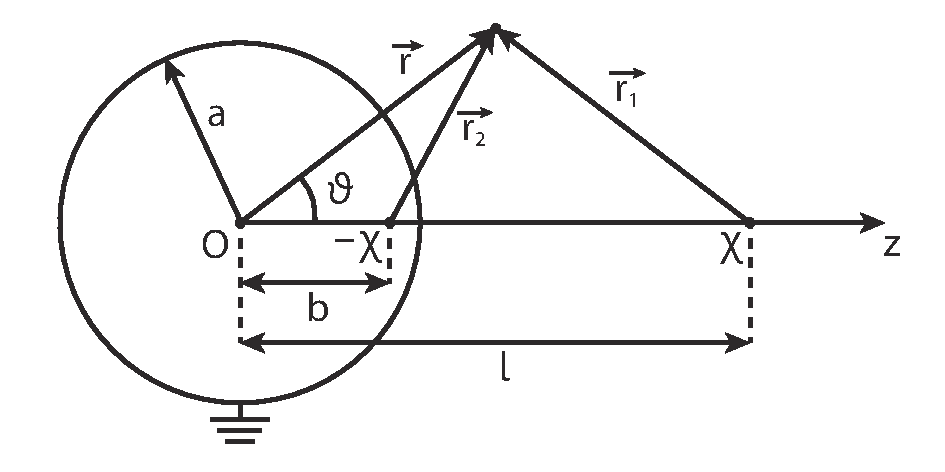
\includegraphics[width=\textwidth]{3-3}
\end{minipage}
\begin{minipage}{.46\textwidth}
    Для решения задачи воспользуемся методом изображений.
    
    В виду того, что цилиндр заземлен, внутри цилиндра поля нет:
    \( E_{in} = 0 \), \( \phi_{in} = \const \).
    
    Вне цилиндра поле создается заряженной нитью \( \chi \) и ее изображением,
\end{minipage}
находящимся на расстоянии \( b \) от оси цилиндра.
    
Поле \( \vec{E} \) бесконечной заряженной прямой нити имеет вид:
\( E = \cfrac{\chi}{2\pi\Ezero r} \), откуда потенциал:
\( \phi = -\cfrac{\chi}{2\pi\Ezero}\ln r \).

Тогда потенциал вне цилиндра имеет вид:
\[
    \phi_{ex} = -\frac{\chi}{2\pi\Ezero}\left(\ln r_1 - c\ln r_2\right),
\]
где \( c = \const \), \( r_1, r_2 > a \);
\( r_1 = \sqrt{l^2 + r^2 - 2lr\cos\theta} \),
\( r_2 = \sqrt{b^2 + r^2 - 2br\cos\theta} \) -- расстояния от рассматриваемой
точки до нити и ее изображения.

Рассмотрим граничное условие \( \phi\bigl|_{r = a} = 0 \):
\[
    \frac{\chi}{4\pi\Ezero}\Bigl(-\ln\left(l^2 + a^2 - 2al\cos\theta\right) +
    c\ln\left(b^2 + a^2 - 2ab\cos\theta\right)\Bigr) = 0.
\]
    
Перепишем в виде:
\[    
    -\ln l - \ln\left(l + a^2/l - 2a\cos\theta\right) + c\ln b +
    c\ln\left(b + a^2/b - 2a\cos\theta\right) = 0.
\]

Далее \( \ln\left( l + a^2/l - 2a\cos\theta\right) = \ln\left(b + b^2/l -
2a\cos\theta\right) \), и \( l + a^2/l = b + b^2/l \), откуда \( b = a^2/l \).

Определим константу \( c \): \( \ln\left( l + a^2/l - 2a\cos\theta \right) =
c\ln\left( a^2/l + l - 2a\cos\theta \right) \), далее \( 1  = c\cdot 1 \),
следовательно, \( c = 1 \).

Тогда напряженность поля вне цилиндра будет определяться выражением:
\( \vec{E} = -\nabla\phi_2 \).

Радиальная компонента:
\[
    E_r = -\pder{\phi_2}{r} = \frac{\chi}{2\pi\Ezero}
    \left( \frac{r - l\cos\theta}{r_1^2} - \frac{r - \frac{a^2}{l}\cos\theta}
    {r_2^2} \right).
\]

Угловая компонента:
\[
    E_\theta = -\frac{1}{r}\pder{\phi_2}{\theta} = \frac{\sin\theta}{2\pi\Ezero}
    \left( \frac{l}{r_1^2} - \frac{a^2/l}{r_2^2} \right).
\]

Сила, действующая на единицу длины нити равна силе взаимодействия между нитью и
ее изображением:
\[
   F = \frac{\chi^2}{2\pi\Ezero(l - b)} = \frac{\chi^2}{2\pi\Ezero\left( l -
   a^2/l \right)} = \frac{\chi^2l}{2\pi\Ezero(l^2-a^2)}.
\]

\vspace*{2em}
\emph{Ответ:}

\vspace*{-4.5em}
\begin{gather*}
    E_r = \frac{\chi}{2\pi\Ezero}\left( \frac{r - l\cos\theta}{r_1^2} -
    \frac{r - \frac{a^2}{l}\cos\theta}{r_2^2} \right); \\
    E_\theta = \frac{\sin\theta}{2\pi\Ezero}\left( \frac{l}{r_1^2} -
    \frac{a^2/l}{r_2^2} \right); \quad
    F = \frac{\chi^2l}{2\pi\Ezero(l^2-a^2)}.
\end{gather*}

\newpage
%-------------------------------------------------------------------------------
Задача 2.33: \emph{Однородный магнетик имеет форму бесконечно длинного
круглого цилиндра радиуса \( a \), магнитная проницаемость его \( \mu \);
окружающая среда -- воздух. Бесконечный прямолинейный ток проходит в воздухе
параллельно оси магнетика на расстоянии \( l \) от нее. Определить создаваемое
им магнитное поле.}

\vspace*{2em}
\emph{Решение:}

\begin{minipage}{.5\textwidth}
    \includegraphics[width=\textwidth]{3-4}
\end{minipage}
\begin{minipage}{.46\textwidth}
    Рассмотрим задачу в цилиндрических координатах. Тогда напряженность
    магнитного поля будет иметь только одну компоненту -- угловую, которая в
    силу теоремы Стокса будет иметь вид:
    \( \ds H_\alpha = \frac{I}{2\pi r} = -\frac{1}{\mu}\pder{A_z}{r} \).
\end{minipage}

Векторный потенциал будет иметь вид: \( \vec{A} = \left\{0, 0, A_z\right\} \).

Внутри цилиндра: \( \ds A_z^{in} = -\frac{I''\mu}{2\pi}\ln r_1 \).

Вне цилиндра: \( \ds A_z^{ex} = -\frac{I}{2\pi}\ln r_1 - \frac{I'}{2\pi}\ln r_2
- \frac{I'''}{2\pi}\ln r \).

Положим \( I' = k_1I \), \( I'' = k_2I \), \( I''' = k_3I \) и выразим
\( r_1 \) и \( r_2 \) через \( r \):\\ 
\( r_1 = \sqrt{l^2 + r^2 - 2rl\cos\theta} \),
\( r_2 = \sqrt{b^2 + r^2 - 2br\cos\theta} \), тогда векторные потенциалы:
\begin{gather*}
    A_z^{in} = -\frac{\mu k_2I}{4\pi}\ln(l^2 + r^2 - 2rl\cos\theta);\\
    A_z^{ex} = -\frac{I}{4\pi}\ln(b^2 + r^2 - 2br\cos\theta) -
    \frac{k_1I}{4\pi}\ln(l^2 + r^2 - 2rl\cos\theta) - \frac{k_3I}{4\pi}\ln r.
\end{gather*}

Рассмотрим граничные условия. Первое -- \( A_z^{in} = A_z^{ex} \):
\begin{gather*}
    -\frac{\mu k_2I}{4\pi}\ln(l^2 + a^2 - 2al\cos\theta) = -\frac{I}{4\pi}
    \ln(l^2 + a^2 - 2al\cos\theta) - \\ - \frac{k_1I}{4\pi}
    \ln(b^2 + a^2 - 2ab\cos\theta) - \frac{k_3I}{2\pi}\ln r.
\end{gather*}

Упрощая, получим:
\[
    -\mu k_2\ln(l^2 + a^2 - 2al\cos\theta) = -\ln(l^2 + a^2 - 2al\cos\theta) -
    k_1\ln(b^2 + a^2 -2ab\cos\theta) - 2k_3\ln a.
\]

Аналогично предыдущей задаче: \( b = a^2/l \). Тогда:
\begin{gather*}
    2\mu k_2\ln l + \mu k_2\ln(1 + a^2/l^2 - 2a/l\cos\theta) = 2\ln l +
    \ln(1 + a^2/l - 2a/l\cos\theta) + 2k_1\ln a + \\ +
    k_1\ln(1 + a^2/l^2 - a/l\cos\theta) + 2k_3\ln a.
\end{gather*}

Или: \( (\mu k_2 - 1 - k_1)\ln(1 + a^2/l^2 - 2a/l\cos\theta) = 2\ln l +
2(k_1 + k_3)\ln a - 2\mu k_2\ln l \).

Так как зависимость от угла должна отсутствовать, то \( \mu k_2 - 1 - k_1 = 0
\), откуда \( k_1 = \mu k_2 - 1 \).

Рассмотрим теперь второе граничное условие \( \ds -\frac{1}{\mu}
\pder{A_z^{in}}{r}\Biggr|_{r = a} + \pder{A_z^{ex}}{r}\Biggr|_{r = a} =
\frac{I}{2\pi} \): сначала возьмем производные
\[
    \pder{A_z^{in}}{r} = -\frac{\mu k_2I}{4\pi}\frac{2r - 2l\cos\theta}{r_1^2},
    \pder{A_z^{ex}}{r} = -\frac{I}{4\pi}\left(\frac{2r - 2l\cos\theta}{r_1^2}
    + k_1\frac{2r - 2b\cos\theta}{r_2^2} - 2k_3\frac{1}{r}\right);
\]
а затем подставим их в условие:
\[
    \frac{k_2I}{4\pi}\frac{2a - 2l\cos\theta}{r_1^2} - \frac{I}{4\pi}
    \frac{2a - 2l\cos\theta}{r_1^2} - \frac{k_1I}{4\pi}\frac{2a - 2b\cos\theta}
    {r_2^2} - \frac{k_3I}{2\pi}\frac{1}{a} = \frac{I}{2\pi},
\]
откуда
\[
    \frac{k_2}{r_1^2}(a - l\cos\theta) - \frac{1}{r_1^2}(a - l\cos\theta) -
    \frac{k_1}{r_2^2}(a - b\cos\theta) - \frac{k_3}{a} = 1.
\]

Подставляя выражение для \( k_1 \), имеем:
\begin{gather*}
    \frac{k_2}{r_1^2}(a - l\cos\theta) - \frac{1}{r_1^2}(a - l\cos\theta) -
    \frac{\mu k_2 - 1}{r_2^2}(a - b\cos\theta) - \frac{k_3}{a} =  1;\\
    \frac{1}{r_1^2}(a - l\cos\theta)(k_2 - 1) - \frac{1}{r_2^2}(a - b\cos\theta)
    (\mu k_2 - 1) - \frac{k_3}{a} = 1,
\end{gather*}
откуда, так как зависимость от угла должна быть одинаковой,
\[
    \frac{\frac{1}{r_1^2}(a - l\cos\theta)}{\frac{1}{r_2^2}(a - b\cos\theta)} =
    \frac{k_2 - 1}{-\mu k_2 + 1} = 1.
\]

Тогда \( k_2 - 1 = -\mu k_2 + 1 \), откуда \( k_2 = 2/(1 + \mu) \). Подставляя
в выражение для \( k_1 \), имеем: \( k_1 = 2\mu/(1 + \mu) - 1 \), откуда
\( k_1 = \frac{\mu - 1}{\mu + 1} \).

Для нахождения коэффициента \( k_3 \) запишем циркуляцию вектора \( \vec{H} \)
по контуру радиуса \( b < R < a \):
\( \ds \oint\vec{H}\cdot\d\vec{l} = I'' + I''' = 0 \), откуда \( k_3 = -k_1 \).

Таким образом, \( \ds H_\alpha^{in} = -\frac{1}{\mu}\pder{A_z^{in}}{r}; \quad
    H_\alpha^{ex} = -\pder{A_z^{ex}}{r} \).

\vspace*{1.5em}
\emph{Ответ:}
\vspace*{-2.7em}
\begin{gather*}
    H_\alpha^{in} = \frac{2I}{2\pi(\mu + 1)}\frac{r - l\cos\theta}{r_1^2}; \\
    H_\alpha^{ex} = \frac{I}{2\pi}\frac{r - l\cos\theta}{r_1^2} +
    \frac{(\mu - 1)I}{2\pi(\mu + 1)}\frac{r - b\cos\theta}{r_2^2} -
    \frac{(\mu - 1)I}{2\pi(\mu + 1)}\frac{1}{r}.
\end{gather*}
\end{document}
